% Submission candidate (2026-11-23), not uploaded. Every number must trace to a file in runs/, reports/ or docs/.
\documentclass[11pt]{article}
\usepackage[margin=1in]{geometry}
\usepackage{graphicx,booktabs,amsmath,longtable,hyperref}
\title{Does Learning to Repair a Drawn Graph Teach a Small VLM to Read It?\\
\large A verified benchmark with answer-flipping twins}
\author{Yi\u{g}it Efe Erdo\u{g}mu\c{s}\\{\normalsize Independent researcher}
\and Yi\u{g}it \c{C}er\c{c}i\\{\normalsize Y{\i}ld{\i}z Technical University}}
\date{}
\begin{document}
\maketitle

\begin{abstract}
% written by scripts/paper_framing.py (rule framing-v2, chosen after reading; see sections/why.tex);
% the pre-registered finding-v1 text (scripts/paper_finding.py) is kept in reports/final/abstract.tex
\IfFileExists{../reports/final/framing_abstract.tex}{% generated by scripts/paper_framing.py, rule framing-v2 (chosen after reading, see DECISIONS 2026-11-23T20:30Z); do not edit
We introduce a procedural benchmark of drawn directed graphs with exact labels, a verifier that accepts every optimal repair edit, and answer-flipping twins that cap any image-blind predictor at $0.50$ per task, and use it to test whether training a small vision-language model only to repair drawings improves its answers to reachability and edge-criticality questions more than training it on those questions directly. On an adapted $500$-graph VGCure evaluation (drawings by other authors in a style none of our adapters saw, with our prompts, images scaled to our input size and strict scoring), the repair-trained adapter (arm~D) answers edge-existence and reachability questions better than direct question-answer fine-tuning (arm~B): the difference is $+0.056$ (95\% interval [$+0.038$, $+0.075$], mean of 3 seeds, above zero at every seed). On our own pre-registered locked test, which decides the hypothesis, D does worse than B: D$-$B is $-0.105$ (95\% interval [$-0.117$, $-0.093$]), so the hypothesis is not supported at this scale. The loss is confined to edge criticality, a task VGCure does not contain, where D answers \emph{true} to 79\% of the questions (true is right for half); the VGCure gain comes mostly from false edge claims and unreachable pairs, which D rejects more often than B. A parse-then-solve arm, which reads the graph with a separately trained extraction adapter, performs best on our benchmark (E$-$B $+0.065$) but scores $0.092$ below direct question-answer fine-tuning on VGCure, where its parser gives no usable graph for 7\% of the images. This is a pilot-scale study: all adapters were trained on $512$ synthetic root graphs with one 2B base model (Qwen3.5-2B, LoRA), and nothing here measures real diagrams.
}{%
\IfFileExists{../reports/final/abstract.tex}{% generated by scripts/paper_finding.py, rule finding-v1, from reports/final/final_primary.json; do not edit
We introduce a procedural benchmark of drawn directed graphs with exact labels, a verifier that accepts every optimal repair edit, and answer-flipping twins that cap any image-blind predictor at $0.50$ per task, and use it to ask whether training a small vision-language model to repair a drawing teaches it to answer reachability and edge-criticality questions it was never trained on. Repair training (arm~D) did worse than the reference fine-tuning arm on the pre-registered six-cell statistic; the hypothesis is not supported at this scale. On the locked test the difference D$-$B is $-0.105$ (95\% interval [$-0.117$, $-0.093$], mean of 3 seeds). This is a pilot-scale study: all adapters were trained on $512$ synthetic root graphs with one 2B base model (Qwen3.5-2B, LoRA), and nothing here measures real diagrams.
}{%
DRAFT. To be written after the main experiments. No result is claimed yet.}}
\end{abstract}

% Introduction. Written before the main experiments: it states the question, the design and
% what the paper provides, and claims no model result. tests/test_paper_intro.py checks that
% it cites only bibliography keys, quotes no measured number, and makes no result claim.
% The final paragraph is to be rewritten once M5/M6 results exist.
\section{Introduction}
\label{sec:intro}

Vision-language models (VLMs) answer many questions about natural images, yet questions
about drawn structure, such as whether one node of a diagram can reach another, remain hard
for them~\cite{mcdgraph,graphverse}. Probing suggests the needed information is often
present in their representations even when the answer is wrong~\cite{signals}. A common
remedy is supervised fine-tuning on the questions themselves or on structural auxiliary
tasks such as describing or completing the graph~\cite{mcdgraph}.

We ask whether a different signal helps: \emph{learning to repair} a drawing. A repair task
gives the model a drawn directed graph and reachability goals and asks for the smallest
edge edit that satisfies them. Producing a correct edit requires reading which edges exist
and which paths depend on which edge; unlike a yes/no answer, the edit can be checked
exactly and leaves little room for guessing. If repair training builds a usable internal
reading of the graph, it should transfer to questions the model was never trained to
answer, such as reachability and edge criticality.

Testing this claim fairly needs two things that the graph-image benchmarks we reviewed
(Section~\ref{sec:related}) do not provide together. First, labels and repair answers must be exact, and the verifier must
accept every optimal edit, not one reference answer. Second, the evaluation must rule out
answers that ignore the image. We build a procedural benchmark with an exact solver, an
independent reference check and \emph{answer-flipping twins}: every question is asked on
two drawings that differ by one edge and have opposite answers, so a predictor that does
not use the image scores at most $0.50$ per task, and answering both twins correctly shows
that the deciding edge was used (Fig.~\ref{fig:twins}).

On this benchmark we compare, on the same base model with LoRA~\cite{lora} and matched
samples, root graphs and images, a repair-trained arm against question-answer training on
the target questions and against structural fine-tuning in the style of
MCDGraph~\cite{mcdgraph}. Oracle conditions that give the true graph as text, and a
parse-then-solve arm in the spirit of describe- or recover-then-compute
methods~\cite{visiongraph,vgcompiler}, help separate failures of reading the drawing from failures of
reasoning about it, within limits we state (the text oracle also changes the input format). All splits are grouped by root graph with no isomorphic graph shared across
splits, and the test splits, including held-out styles, families and sizes, are opened once.

\paragraph{Contributions.}
(i)~A verified generator and benchmark for drawn directed graphs with exact labels,
answer-flipping twins, invariance pairs and leakage-free splits (Section~\ref{sec:benchmark}).
(ii)~A pre-specified, exposure-matched protocol for testing whether edit training transfers
to non-edit questions in a small VLM (Sections~\ref{sec:setup} and~\ref{sec:analysis}).
(iii)~Oracle-graph and parse-and-solve conditions that help separate perception errors from
reasoning errors, with their limits stated. (iv)~A pre-registered external check on drawings by other authors
(VGCure) and an item-level account of why it and our locked test disagree about repair
training (Sections~\ref{sec:external} and~\ref{sec:why}). (v)~A record of what did not work
during development (Section~\ref{sec:negative}). Code and data: \url{https://github.com/efeerdogmus0/trace-graph-repair}.
% Main findings paragraph: scripts/paper_framing.py (rule framing-v2, chosen after reading); the pre-registered
% finding-v1 paragraph (scripts/paper_finding.py) is kept in reports/final/intro_finding.tex.
\IfFileExists{../reports/final/framing_intro.tex}{% generated by scripts/paper_framing.py, rule framing-v2 (chosen after reading, see DECISIONS 2026-11-23T20:30Z); do not edit
\paragraph{Main findings.} On an adapted $500$-graph VGCure evaluation (drawings by other authors in a style none of our adapters saw, with our prompts, images scaled to our input size and strict scoring), the repair-trained adapter (arm~D) answers edge-existence and reachability questions better than direct question-answer fine-tuning (arm~B): the difference is $+0.056$ (95\% interval [$+0.038$, $+0.075$], mean of 3 seeds, above zero at every seed). The lead comes from both tasks: edge existence $+0.049$ and reachability $+0.063$. On our own pre-registered locked test, which decides the hypothesis, D does worse than B: D$-$B is $-0.105$ (95\% interval [$-0.117$, $-0.093$]), so the hypothesis is not supported at this scale. Section~\ref{sec:why} traces the disagreement: on our test D's deficit is in the critical-edge task, where it answers \emph{true} to 79\% of the questions, while its reachability is level with B's; on VGCure, which has no critical-edge items, D gains on false edge claims and unreachable pairs. This is a pilot-scale study: all adapters were trained on $512$ synthetic root graphs with one 2B base model (Qwen3.5-2B, LoRA), and nothing here measures real diagrams. Both evaluations were fixed before any of their outputs existed; giving the external result this place in the abstract and introduction was decided after both were read, while the wording rule fixed in advance put only the locked-test statistic here (Section~\ref{sec:why}). Per-split, per-task and secondary comparisons are in Section~\ref{sec:test-results}.
}{%
\IfFileExists{../reports/final/intro_finding.tex}{% generated by scripts/paper_finding.py, rule finding-v1, from reports/final/final_primary.json; do not edit
\paragraph{Main finding.} Repair training (arm~D) did worse than the reference fine-tuning arm on the pre-registered six-cell statistic; the hypothesis is not supported at this scale. On the locked test the difference D$-$B is $-0.105$ (95\% interval [$-0.117$, $-0.093$], mean of 3 seeds). This is a pilot-scale study: all adapters were trained on $512$ synthetic root graphs with one 2B base model (Qwen3.5-2B, LoRA), and nothing here measures real diagrams. Per-split, per-task and secondary comparisons are in Section~\ref{sec:test-results}.
}{}}


% Related work. Every claim about another paper comes from docs/related_work.md (pages read
% 2026-11-09/10); bibliographic data from docs/sources/arxiv_bib_2026-11-12.xml (arXiv API).
% The overlap search was about eight queries (2026-11-09), extended on 2026-11-15 by 14 fixed
% arXiv API queries (scripts/overlap_search.py, docs/sources/overlap_2026-11-15/); still not an
% exhaustive negative. Claims about the 2026-11-15 additions come from their arXiv abstracts only.
\section{Related Work}
\label{sec:related}

\paragraph{Visual graph understanding.}
VGCure and its MCDGraph training recipe~\cite{mcdgraph} benchmark large VLMs on
fundamental questions about drawn graphs and improve them with structural fine-tuning:
masked graph infilling, contrastive graph discrimination (two images, same graph or not)
and graph description, applied with LoRA to 7--8B models. Our arm~C follows this recipe
at matched exposure. GraphVerse~\cite{graphverse} is a broader benchmark of single- and
paired-image graph tasks and trains Qwen3-VL models; its ``editing'' denotes
topology-preserving perturbations of the input, not an edit the model outputs, and
reachability is not one of its tasks. Neither work asks the model to \emph{produce} an
edge edit that satisfies a goal, nor compares edit training with question-answer training
on the same graphs. Probing work~\cite{signals} reports that node and edge information
is linearly decodable from VLM representations of diagrams even where question answering
fails, which motivates our attempt to separate perception from reasoning with oracle-graph and
parse-and-solve conditions.

\paragraph{Recover the graph, then compute.}
Our arm~E, which parses the drawing into an edge list and answers with an exact solver,
has close precedents. VisionGraph~\cite{visiongraph} pairs a benchmark of graph-theory
problems on images with a description--program--reasoning chain and reports that
perception of the graph structure limits all tested models. VGCompiler~\cite{vgcompiler}
trains an 8B VLM with reinforcement learning to recover an explicit graph representation
and compile the question into an executable graph operation. Knossos and
Ariadne~\cite{knossos} study complete diagram-to-graph extraction with exactly aligned
synthetic annotations. MapReason-OSM~\cite{mapreason} scores structured decisions on
rendered maps against a hidden graph with exact oracles. We do not claim parse-and-solve
as a contribution; arm~E is the reference that tells whether a gain from edit training
exceeds what explicit graph recovery already gives at the same base and data.

\paragraph{Minimal edits as a training signal.}
Controlled minimal edits of natural images have been used as fine-grained supervision,
with a consistency objective over edited pairs~\cite{med} or as counterfactual
contrastive signal~\cite{cfvlm}. Diagram editing also appears as one stage in a
geometry-reasoning training pipeline~\cite{geoweave}. These works edit natural images or
use editing alongside other stages; none isolates whether learning to edit transfers to
non-edit questions, and none has an exact verifier that accepts every optimal edit.
Our answer-flipping twins are minimal edits used for \emph{evaluation}: each pair differs
by one edge and has opposite answers, bounding an image-blind model at 0.50.

\paragraph{Parameter-efficient adaptation.}
All trained arms use LoRA~\cite{lora} on the same base, so differences come from the
training data, not the adaptation method.


% Sources: docs/datasheet.md, docs/datasheet_pilot_stats.md (generated), docs/protocol.md,
% reports/pilot*/validation.json, paper/figures/fig1.json (generated by scripts/paper_figure.py).
\section{Benchmark}
\label{sec:benchmark}

\begin{figure*}[t]
\centering
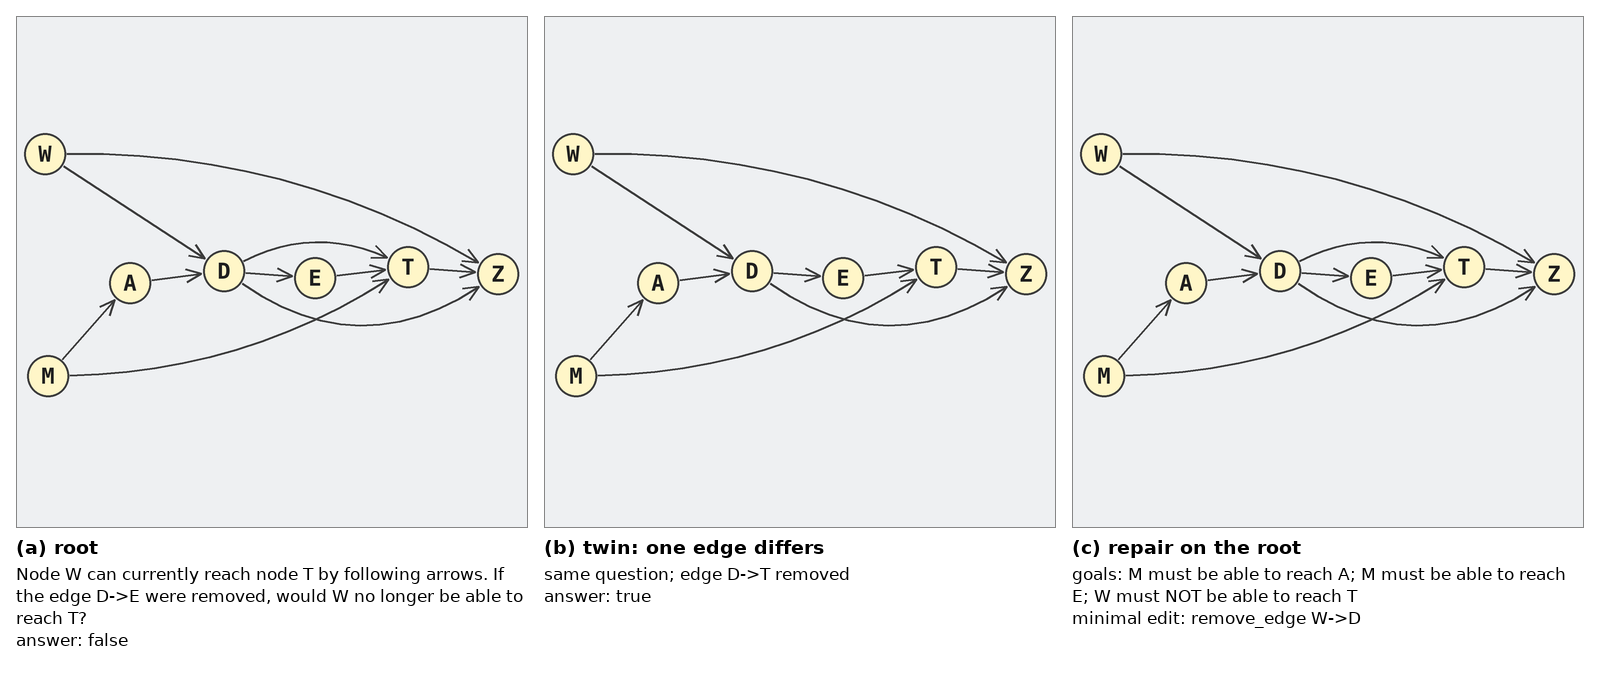
\includegraphics[width=\textwidth]{figures/fig1.png}
\caption{One root graph from the pilot dev split (group \texttt{gabe1987fbac2}).
(a) Critical-edge question; removing $D\!\to\!E$ leaves the path $W\!\to\!D\!\to\!T$, so the
answer is \emph{false}. (b) The answer-flipping twin: the same text with edge $D\!\to\!T$
absent; now the answer is \emph{true}. (c) The repair task on the root image: the only
minimal edit is removing $W\!\to\!D$. Questions, answers and the differing edge are read
from the dataset by \texttt{scripts/paper\_figure.py} and checked against an independent
reference solver in \texttt{tests/test\_paper\_figure.py}.}
\label{fig:twins}
\end{figure*}

\paragraph{Graphs and drawings.}
Each instance is a $512\times512$ drawing of a weakly connected, simple directed graph
without antiparallel edges. Training and in-distribution graphs come from three families
(\texttt{layered\_dag}, \texttt{tree\_plus}, \texttt{sparse\_random}), are placed by one of
four layouts and drawn in one of three styles. Every drawing passes geometric readability
rules (node spacing, edges clear of other nodes, recorded crossings) and a pixel read-back
against the intended drawing.

\paragraph{Tasks.}
The main tasks are \emph{reachability}, \emph{critical edge} (would removing a given edge
disconnect $s$ from $t$?) and \emph{minimal graph repair}: given reachability goals and a
list of edges that may be added (any present edge may be removed), output at most one edit,
or \texttt{unchanged}, or \texttt{impossible}. The repair verifier applies the answer to the
true graph and accepts every minimal solution. Edge existence, shortest-path length and
full graph extraction are secondary tasks. Answers are single JSON objects scored strictly.

\paragraph{Exact labels.}
Labels come from an exact solver and are re-checked by an independent brute-force reference
(transitive closure by Floyd--Warshall). The validator for the pilot build ran 249{,}139
checks with 0 errors; the locked test build ran 258{,}984 checks with 0 errors.

\paragraph{Answer-flipping twins.}
Every main-task question appears with two images that differ by exactly one edge and have
opposite answers (Fig.~\ref{fig:twins}a,b). A predictor that ignores the image therefore
scores at most $0.50$ on each main task, and the share of twin pairs answered correctly on
\emph{both} images measures whether the model uses the edge at all. About a quarter of root
graphs also receive a relabelled and a restyled copy with the same answer (invariance pairs).

\begin{table}[h]
\centering
% Generated by scripts/modelfree_table.py from reports/*/validation.json; do not edit by hand.
\begin{tabular}{lrccccccc}
\toprule
 & & \multicolumn{2}{c}{reachability} & \multicolumn{2}{c}{critical edge} & \multicolumn{3}{c}{minimal repair} \\
\cmidrule(lr){3-4}\cmidrule(lr){5-6}\cmidrule(lr){7-9}
split & roots & const. & text & const. & text & const. & heur. & text \\
\midrule
pilot train & 512 & 0.500 & 0.500 & 0.500 & 0.500 & 0.250 & 0.2637 & 0.500 \\
pilot dev & 200 & 0.500 & 0.500 & 0.500 & 0.500 & 0.250 & 0.2625 & 0.500 \\
test ID & 200 & 0.500 & 0.500 & 0.500 & 0.500 & 0.250 & 0.2650 & 0.500 \\
test style OOD & 200 & 0.500 & 0.500 & 0.500 & 0.500 & 0.250 & 0.2700 & 0.500 \\
test structure OOD & 200 & 0.500 & 0.500 & 0.500 & 0.500 & 0.250 & 0.2650 & 0.500 \\
test combined OOD & 100 & 0.500 & 0.500 & 0.500 & 0.500 & 0.250 & 0.2500 & 0.500 \\
diagnostic family OOD & 100 & 0.500 & 0.500 & 0.500 & 0.500 & 0.250 & 0.2500 & 0.500 \\
diagnostic size OOD & 100 & 0.500 & 0.500 & 0.500 & 0.500 & 0.250 & 0.2600 & 0.500 \\
\bottomrule
\end{tabular}

\caption{Model-free baselines per split, computed by the validator with the real scorer from labels and
instructions alone (no model is involved). \emph{const.}: the better of the two constant answers
(\emph{true}/\emph{false}; for repair \emph{unchanged}/\emph{impossible}), i.e.\ the majority-class
score. \emph{heur.}: the best of three text heuristics for repair (add the edge the goal names, add the
first listed edge, remove the edge named by the first forbidden pair). \emph{text}: the best accuracy of
any predictor that sees the instruction but not the image. Counted on the root and edited images only.}
\label{tab:modelfree}
\end{table}

\paragraph{Model-free baselines.}
Table~\ref{tab:modelfree} gives the scores reachable without the image on every split, including the
locked ones. Both Boolean main tasks are exactly balanced, so a constant answer scores $0.500$; on repair
a constant status scores $0.250$ and no text heuristic exceeds $0.27$. The text-only ceiling is $0.500$
on all three main tasks in every split. These are properties of the builds, fixed when the data was
generated; they are the floor against which every model score in this paper should be read.

\paragraph{Splits without leakage.}
The split unit is the root graph and everything derived from it; no two graphs in
different groups are isomorphic. The locked test build adds held-out drawing styles,
held-out graph families with larger graphs, and their combination; a second locked build
separates the family shift from the size shift. Test labels are guarded in code and opened
once, for the final evaluation.

\paragraph{Reproducibility.}
The content digest (graphs, labels, instructions) was identical on macOS (Python~3.9 and~3.12)
and Linux (Python~3.13); PNG bytes differ between machines through font
rasterisation, so images are rebuilt from the generator and checked by content.

\begin{table}[h]
\centering
\begin{tabular}{lrrr}
\toprule
build / split & root graphs & images & samples \\
\midrule
pilot train & 512 & 2{,}207 & 5{,}092 \\
pilot dev & 200 & 869 & 2{,}012 \\
locked test (ID, style, structure, combined) & 200/200/200/100 & 3{,}078 & 7{,}006 \\
locked diagnostic (family-only, size-only) & 100/100 & 869 & 1{,}978 \\
\bottomrule
\end{tabular}
\caption{Pilot-scale builds (\texttt{docs/datasheet\_pilot\_stats.md}, \texttt{docs/datasheet.md}).
The main build (planned: about 5{,}000 training roots, 7--12 nodes) was not built (Section~\ref{sec:setup}).}
\end{table}


% Sources: docs/protocol.md (v1.0 as executed; sections 1-6 frozen, scripts/protocol_freeze.py), src/trace_vr/arms.py,
% scripts/train_arm.py (constants LR, WARMUP, R, TARGETS), src/trace_vr/model.py (BASE_ID,
% BASE_REVISION), src/trace_vr/parse_solve.py, src/trace_vr/token_budget.py,
% src/trace_vr/bootstrap.py, docs/exposure_pilot_train.md (generated by scripts/exposure.py).
% tests/test_paper_setup.py re-checks every number below against those files.
% manifests/pilot.json, manifests/pilot_test.json (Scale paragraph).
% No model result is stated in this section.
\section{Setup}
\label{sec:setup}

\paragraph{Hypothesis.}
H1: training a small VLM only to output minimal repair edits on drawn directed graphs
improves its accuracy on \emph{non-edit} relational questions (reachability, critical edge)
about unseen root graphs more than fine-tuning the same base on those questions directly,
or on structural graph tasks, at equal samples and images. H0: any gain is explained by
generic fine-tuning, extra data, output length, resolution or evaluation shortcuts.
Reachability appears inside the repair goals, so the claim concerns transfer from an edit
objective to questions, not the learning of a new concept.

\paragraph{Base model and adaptation.}
All arms start from \texttt{Qwen/Qwen3.5-2B} at a pinned revision (\texttt{15852e8c}). Trained
arms use LoRA with rank $r=16$, $\alpha=16$, no dropout, on the attention, linear-attention
and MLP projections of the language model; the vision encoder is frozen. Optimisation:
AdamW, learning rate $2\times10^{-4}$, weight decay $0.01$, linear warm-up over $3\%$ of the
updates then linear decay, gradient clipping at $1.0$, batch size 1 with 4-step gradient
accumulation, loss on the answer tokens only. Every image is $512\times512$ pixels and costs
256 image tokens for every arm and split. Training seeds are 3407, 2027 and 9173.

\paragraph{Arms.}
\begin{description}
\item[A, frozen base.] No training; same parser as every other arm. With the prompt every
  other arm sees, the base reasons in prose and runs out of tokens, so its prompt was chosen on
  development data by a rule fixed beforehand (highest strict non-edit macro accuracy at the
  variant's own token limit, ties to the common prompt). On 20 development roots (80 non-edit
  questions) the common prompt scored $0.1375$ at 768 new tokens (lenient parse $0.6125$,
  truncation up to $0.90$ per task); one added sentence (``Do not explain your reasoning.
  Reply with the JSON object only.'') scored $0.6000$ after the question and $0.6250$ as a
  system message, both at 96 new tokens with no truncation. Arm A therefore uses the system
  message at 96 new tokens. The two short variants differ by two questions; the choice
  follows the rule and is not evidence that one is better. A is a reported floor, not a
  compared arm.
\item[B, QA-SFT.] One non-edit twin pair per root graph, alternating reachability and
  critical-edge questions.
\item[C, structural SFT.] An adaptation inspired by MCDGraph~\cite{mcdgraph} (not a
  reproduction): on exactly the images D sees, a fixed cycle of graph description (list every
  node and edge), masked infilling (name the withheld third of a listed edge set) and
  one-image graph matching (is this edge list exactly the drawn graph? negatives differ by one
  edit). The edge lists in C's prompts are its declared extra training input.
\item[D, TRACE.] Minimal repair only: the root image and its repair twin of every root
  graph, answer \texttt{edited} with one edit, \texttt{unchanged} or \texttt{impossible}.
\item[E, parse and solve.] An extraction adapter, \texttt{C\_desc} (the same base with LoRA,
  trained per seed only on the graph-description task, list every node and edge, on the images
  D sees), transcribes each image once; fixed cleaning rules, decided before any E output existed, turn it into a graph on which the exact
  solver answers every question. E is scored against the true graph like every other arm.
\end{description}
D2 (D with an auxiliary ``does the goal hold after this edit?'' task) is the first of the two
revisions the protocol allows after a failed pilot. Because removal edits make that task close
to the critical-edge question, D2 is not a pure transfer test and is reported separately.

\paragraph{Matched exposure.}
Per epoch on the pilot training split every trained arm sees the same 1{,}024 samples from
the same 512 root graphs and 1{,}024 distinct images, and all arms train for the same number
of epochs. Text length is not equalised; it is reported (Table~\ref{tab:exposure}). C and D2
use exactly D's images; B uses the same root graphs but other twins and shares 546 of D's
1{,}024 images.

\begin{table}[h]
\centering
\small
\begin{tabular}{lrrrrr}
\toprule
arm & samples & root graphs & images & instruction tokens & target tokens \\
\midrule
B  & 1{,}024 & 512 & 1{,}024 &  73{,}216 &  5{,}120 \\
C  & 1{,}024 & 512 & 1{,}024 &  92{,}146 & 28{,}592 \\
D  & 1{,}024 & 512 & 1{,}024 & 195{,}542 & 16{,}384 \\
D2 & 1{,}024 & 512 & 1{,}024 & 148{,}410 & 10{,}764 \\
\bottomrule
\end{tabular}
\caption{Training exposure per epoch on the pilot training split (generated by
\texttt{scripts/exposure.py}; text tokens from the base tokenizer, without the chat template).
Image tokens are $256$ per sample for every arm.}
\label{tab:exposure}
\end{table}

\paragraph{Scale.}
This is a pilot-scale study. Every trained adapter saw 512 training root graphs with 5 to 10
nodes for 3 epochs, and every choice was made on 200 development roots. The protocol planned a
main build of about 5{,}000 training roots and locked splits of 500, 500, 500 and 250 roots;
that build was not run. The locked test has 200, 200, 200 and 100 root graphs (ID, style-OOD,
structure-OOD, combined-OOD); its structure-OOD and combined-OOD graphs have 11 to 16 nodes.
Every statement in this paper is a statement about adapters of this size.

\paragraph{Decoding and scoring.}
Decoding is greedy. The primary score is strict: after trimming whitespace and at most one
Markdown code fence the response must be exactly one JSON object with the declared keys;
prose or a reasoning preamble is a format failure and counts as wrong. A lenient score (last
balanced JSON object) is reported next to it for every arm, never instead of it. The token
limit per arm is fixed by a rule set before measurement: one greedy development run at 768 new
tokens gives every shorter limit as a prefix, and the arm uses the smallest of 96, 192, 384
and 768 at which no task exceeds $2\%$ truncation.

\paragraph{Statistic and interpretation rules.}
The primary statistic is the unweighted mean of six accuracies, \{reachability, critical
edge\} $\times$ \{ID test, style-OOD test, structure-OOD test\}, over root and edited images.
Intervals come from a paired bootstrap over root graphs (2{,}000 resamples, fixed seed). Fixed
in advance: a clear positive requires D to exceed the stronger of B and C (chosen on
development data) by about 5 points, not driven by one style or seed; a drop of more than 2
points in either task mean rules out ``general improvement''; if E beats D this is reported.
Test labels are locked in code and opened once, after every choice above is frozen on
development data.


% Sources: docs/protocol.md (sections 5-7), src/trace_vr/analysis.py (FACETS, answer_bias,
% pair_table, invariance_table, density_window), src/trace_vr/arms.py (eval_samples,
% invariance_samples), scripts/colab/final_eval.sh, reports/density/pilot_dev.json,
% reports/parse_solve/sensitivity_dev.json. tests/test_paper_analysis.py re-checks every number.
% Written before any main run. It fixes what is computed, not what will be found.
\section{Analysis plan}
\label{sec:analysis}

Everything in this section is fixed before the main runs and computed by committed scripts
from per-sample correctness flags, so no analysis needs the raw responses or a second look
at the test labels. Only the primary statistic (Section~\ref{sec:setup}) decides the
hypothesis; every quantity below is reported for every arm and seed, labelled secondary, and
is not corrected for multiple comparisons because no claim rests on it alone.

\paragraph{Cells and task means.}
Each of the six accuracies behind the primary statistic is shown with its own paired
interval, together with the reachability and critical-edge means and, for repair, status
accuracy, valid-edit rate and minimal-repair accuracy. Format failures (strict) and the
lenient score are reported per task.

\paragraph{Twin pairs and answer bias.}
For every answer-flipping twin pair we count both right, one right and both wrong. A model
that ignores the differing edge gets at most one of the two right, so ``both right'' is the
measure of whether it uses the edge. For yes/no tasks we report how often the model answered
true next to how often true was correct; with valid format this is recovered exactly from the
flags and the labels.

\paragraph{Invariance pairs.}
Some root questions are repeated on a relabelled copy and on a restyled copy of the same
graph with the same answer. The copies are scored in a separate run on the same roots and
paired with the root answers afterwards; we report both right and how often the two answers
have the same correctness. On the pilot development split this adds 212 copies (53 per pair
kind and task) to 1{,}200 main samples, and 884 copies over the six locked test splits.

\paragraph{Slices.}
Accuracy is broken down by true answer, image variant (root or edited), graph family, size
bucket ($\le 8$, 9--12, $\ge 13$ nodes), layout and style. The structure-OOD cell changes
family and size together, so the separate family-only and size-only splits are reported as a
$2\times2$ table next to the primary statistic, never inside it. Because layout rejection
leaves large graphs sparser, size-OOD is also scored on a density-matched slice: roots whose
edges per node lie inside the central 5--95\% (nearest rank) of the 512 training roots,
$[0.875, 1.667]$. The slice is shown next to the full split, never instead of it.

\paragraph{Perception or reasoning.}
Two diagnostics help separate reading the drawing from reasoning about it. (i) Oracle text: an
adapter trained with the same recipe answers with the true edge list in the prompt and a blank
image, compared with the image-mode result of the arm (for D these are two checkpoints trained
separately with the same recipe); it is reported outside the main table and is not a clean upper bound with perception
removed, because arms trained only on images meet an unfamiliar input format (B scores lower
with the edge list as text than with the image, Section~\ref{sec:negative}). (ii) Arm E is scored with node and edge precision and recall and
direction accuracy of its extraction, next to a model-free curve of how the exact solver
degrades when its input graph is wrong. On the 200 pilot development roots, dropping one or
two true edges per image lowers the non-edit macro accuracy of exact solving from $1.0$ to
$0.8075$ and $0.685$; reversing one or two edges lowers it to $0.73$ and $0.585$. Parse and
solve is therefore only as good as an almost error-free extraction, which is why E is reported
with its extraction quality and not only its answers.

\paragraph{Seeds and decision order.}
Each of the three training seeds is shown individually and pooled; a positive reading must
hold in each seed. The reference baseline (the stronger of B and C), the token limits and the
prompt of the frozen base are chosen on development data and written to the decision log
before the locked splits are evaluated, once, by \texttt{final\_eval.sh}.


\section{Pilot results (development split)}
\label{sec:results}
% Numbers come from reports/pilot/results_dev.json and runs/go_no_go_rev1.json
% and reports/pilot/seeds_dev_interim.json (checked by tests/test_paper_results.py and
% tests/test_paper_seeds.py). Locked-test numbers are not typed here; they are in
% test_results.tex, generated from reports/final/ (opened 2026-11-22).

Table~\ref{tab:results-dev} lists every trained arm on the 200 development root graphs of the
pilot build, image input, strict scoring, one training seed. Intervals are 95\% root-graph
bootstrap intervals (2000 replicates); differences are paired on the same root graphs against
B trained on the same machine (Kaggle T4). These are pilot numbers on the split used for
decisions, not test results.

\begin{table}[t]
\centering\small
% Generated by scripts/results_table.py; do not edit by hand.
\begin{tabular}{lccccc}
\toprule
Arm & Repair & Reach. & Crit. edge & Non-edit macro & $\Delta$ macro vs B\_kaggle \\
\midrule
B\_kaggle & 0.292 & 0.830 & 0.762 & 0.796 & ref \\
C\_kaggle & 0.255 & 0.700 & 0.375 & 0.537 & $-0.259$ {\scriptsize[$-0.294$, $-0.224$]} \\
E\_kaggle & 0.830 & 0.935 & 0.833 & 0.884 & $+0.088$ {\scriptsize[$+0.054$, $+0.121$]} \\
B\_colab & 0.295 & 0.845 & 0.770 & 0.807 & $+0.011$ {\scriptsize[$-0.006$, $+0.028$]} \\
D\_colab & 0.545 & 0.840 & 0.502 & 0.671 & $-0.125$ {\scriptsize[$-0.153$, $-0.099$]} \\
D2\_kaggle & 0.500 & 0.770 & 0.495 & 0.633 & $-0.164$ {\scriptsize[$-0.190$, $-0.138$]} \\
\bottomrule
\end{tabular}

\caption{Development-split accuracy (pilot build, 200 root graphs, one seed). Reach.\ =
reachability, Crit.\ edge = critical edge; the non-edit macro averages these two. The last
column is the paired difference in non-edit macro accuracy to B\_kaggle with its 95\% interval.
The suffix names the machine the arm was trained on.}
\label{tab:results-dev}
\end{table}

\paragraph{Repair training does not transfer to the non-edit questions.}
Both repair-trained arms are below B on their own machine: D by $-0.136$
($-0.163$ to $-0.109$) and the revised D2 by $-0.164$ ($-0.190$ to $-0.138$) in non-edit
macro accuracy; no bootstrap replicate of either difference was above zero. Retraining B on the
second machine moved it by $-0.011$ ($-0.028$ to $+0.006$), so the gap is not a machine effect.
By the rule fixed before this comparison was read (Section~\ref{sec:negative}), the transfer
hypothesis is closed as not supported at pilot scale and the second allowed revision is not spent.

\paragraph{The structural baseline is weaker still.}
C, trained on graph description, masked infilling and graph matching over the same images, reaches
a non-edit macro of $0.537$, $-0.259$ ($-0.294$ to $-0.224$) below B. Its critical-edge
accuracy ($0.375$) is below the balanced chance level, so the structural tasks did not supply
the edge-level reasoning the questions need.

\paragraph{The gaps hold across three training seeds.}
B, C, D and the parser of E were each trained with all three pre-registered seeds on the same machine
(Kaggle T4);
Table~\ref{tab:seeds-dev} pools them. Pooling averages the seeds on the same resampled root graphs
(2000 replicates), so the interval reflects the root graphs, not seed variance; the per-seed gaps
are reported next to it. Pooled over seeds, D is $-0.131$ ($-0.153$ to $-0.110$) and C is
$-0.249$ ($-0.277$ to $-0.222$) below B in non-edit macro accuracy, and every seed-matched gap has
the same sign (D: $-0.136$ to $-0.124$; C: $-0.259$ to $-0.241$). By the rule fixed before the
second seed was read, both are negative readings. The same seed table chose B over C as the
reference baseline for the locked test. The parse-and-solve arm E, whose description parser was
retrained per seed, is $+0.072$ ($+0.042$ to $+0.102$) above B, with every seed-matched gap
positive (E: $+0.061$ to $+0.088$), a clear positive reading by the same rule: on the development
split, transcribing the drawing and solving exactly is the strongest of the four seed-pooled arms.

\begin{table}[t]
\centering\small
% Generated by scripts/seed_table.py; do not edit by hand.
\begin{tabular}{lcccccc}
\toprule
Arm & Seeds & Repair & Reach. & Crit.\ edge & Non-edit macro & $\Delta$ macro vs B \\
\midrule
B & 3 & 0.302 & 0.828 & 0.767 & 0.798 {\scriptsize[0.776, 0.822]} & ref \\
C & 3 & 0.252 & 0.689 & 0.408 & 0.549 {\scriptsize[0.530, 0.569]} & $-0.249$ {\scriptsize[$-0.277$, $-0.222$]} \\
D & 3 & 0.537 & 0.814 & 0.519 & 0.667 {\scriptsize[0.647, 0.686]} & $-0.131$ {\scriptsize[$-0.153$, $-0.110$]} \\
E & 3 & 0.838 & 0.925 & 0.814 & 0.870 {\scriptsize[0.844, 0.894]} & $+0.072$ {\scriptsize[$+0.042$, $+0.102$]} \\
\bottomrule
\end{tabular}

\caption{Development split, pooled over three training seeds (2027, 3407, 9173) per arm, all
trained on Kaggle T4. Task columns are pooled accuracy; brackets are 95\% root-graph bootstrap
intervals of the pooled value; the last column is the pooled paired difference to B.}
\label{tab:seeds-dev}
\end{table}

\begin{figure}[t]
\centering
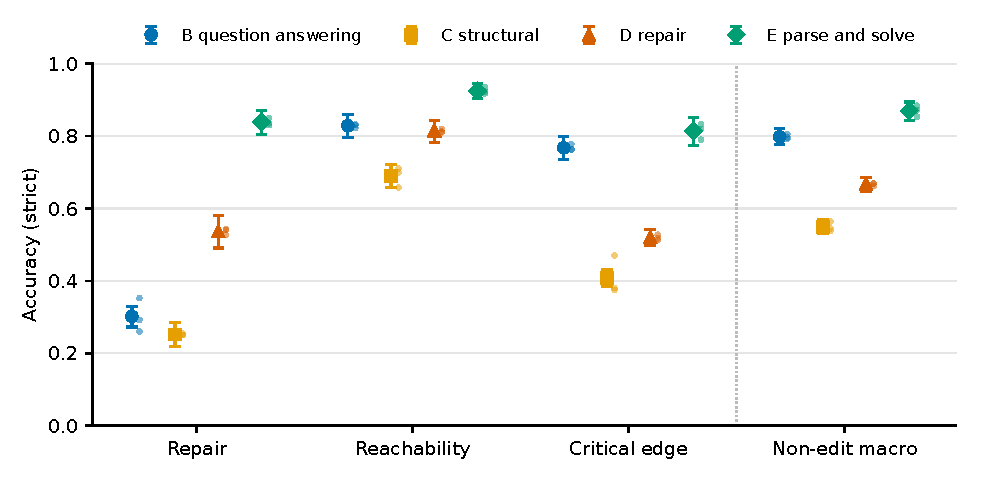
\includegraphics[width=\textwidth]{figures/arms_dev.pdf}
\caption{Development split, the values of Table~\ref{tab:seeds-dev} per task. Marker: accuracy pooled
over the three training seeds; bar: its 95\% root-graph bootstrap interval; small dots: single seeds.
The accuracy axis runs from 0 to 1. Generated from the recorded metrics by \texttt{scripts/dev\_figures.py}.}
\label{fig:arms-dev}
\end{figure}

\paragraph{Cost.}
Figure~\ref{fig:arms-dev} shows the same ordering of the pooled values on every non-edit task. The end-to-end arms cost
about the same to evaluate: on the 1200 development samples one run of B, C or D took $1128.6$ to
$1319.5$ T4 seconds. E took $4141.7$ to $4287.8$ seconds, because it writes out the whole edge list
before the solver answers; its advantage on this split is bought with more than three times the
evaluation time. Training times lie between $1487.7$ and $2079.3$ seconds for all twelve runs.

\begin{figure}[t]
\centering
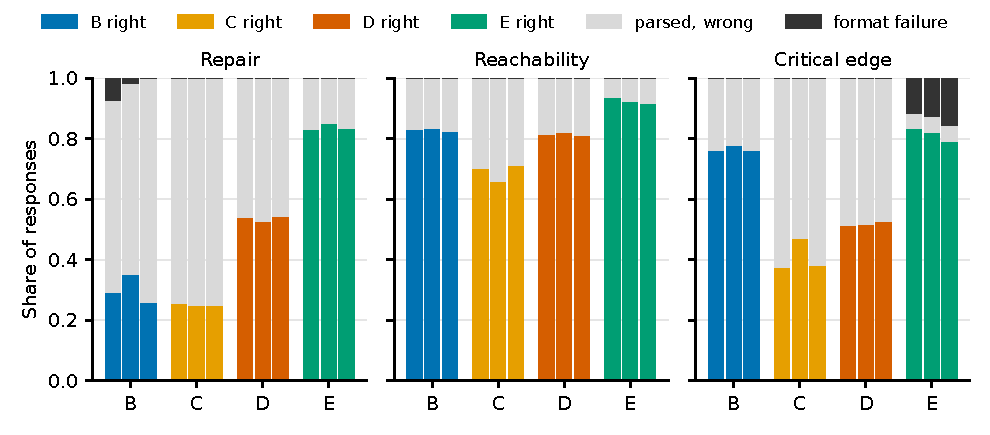
\includegraphics[width=\textwidth]{figures/errors_dev.pdf}
\caption{Development split, what the responses of each run were (one bar per training seed).
Coloured: right under the strict parser; light grey: parsed but wrong; dark: format failure, which
counts as wrong. For E a dark segment is a critical-edge question whose premise fails on the
transcribed graph, so the solver gives no answer. Accuracy and format-failure rate are the recorded
ones; the grey share is their remainder. Generated by \texttt{scripts/dev\_figures.py}.}
\label{fig:errors-dev}
\end{figure}

\paragraph{Error types.}
Figure~\ref{fig:errors-dev} splits the errors of each run. The end-to-end arms almost never fail on
format: C and D have no format failure on any task in any run, and B has none on the two non-edit
tasks and $29$, $7$ and $1$ of $400$ on repair (seeds 3407, 2027, 9173). Their errors are
well-formed wrong answers, and the recorded lenient score equals the strict one on every task in all
nine runs. E is different on one task: for $47$, $50$ and $62$ of its $400$ critical-edge questions per run
the premise fails on the transcribed graph (the source does not reach the target there, or the
queried edge is missing), the solver returns no answer, and the sample is scored as wrong.
These are $47$ of $67$, $50$ of $72$ and $62$ of $84$ of E's critical-edge errors, so most of what E loses there
is a transcription error surfacing as an unanswerable question, not a wrong computation.

\paragraph{Where repair training helps.}
On the repair task itself D ($0.545$) and D2 ($0.500$) are well above B ($0.292$) and C ($0.255$),
so the adapters did learn the training task; the failure is in the transfer.

\paragraph{Parsing the drawing and solving exactly beats every end-to-end arm.}
E uses an adapter trained only to transcribe the drawing as an edge list (same images, same
budget) and answers every question with the exact solver on the transcribed graph. It reaches a
non-edit macro of $0.884$, $+0.088$ ($+0.054$ to $+0.121$) above B, and $0.830$ on repair.
Its transcription is exact for only $359$ of $763$ development images, so the end-to-end arms do not
lose to E because the drawings are unreadable. On the samples whose image E reads exactly, D is
still $-0.148$ ($-0.190$ to $-0.105$) below B, so the gap does not come from drawings that are hard
to transcribe. The split fixed before E was read back (Section~\ref{sec:analysis}) labels this a
reasoning gap; that label uses E's parser as a proxy for how hard a drawing is and does not measure
what the other arms perceived, so it does not by itself rule out a part for perception.


% Locked-test results. Written before any locked-test number was read (2026-11-15).
% Every table is \input from reports/final/<name>.tex, which scripts/final_reports.py writes
% (all-or-nothing, fixed order) once all twelve final kernels are collected. Until then each
% table prints a "pending" line, so the draft compiles and no number is typed by hand.
% tests/test_paper_test_results.py checks the wiring and that this file contains no digits
% outside comments, labels and file names.
\section{Locked-test results}
\label{sec:test-results}

\newcommand{\finaltable}[3]{%
  \IfFileExists{../reports/final/#1.tex}{%
    \begin{table}[t]\centering\small
    \resizebox{\linewidth}{!}{\input{../reports/final/#1.tex}}
    \caption{#2}\label{#3}
    \end{table}}{%
    \par\noindent\emph{Pending: \texttt{\detokenize{reports/final/#1.tex}} is written by
    \texttt{scripts/final\_reports.py} after all locked-test kernels are collected.}\par}}
% final_slices.tex is a longtable (it runs over several pages), so it cannot sit in a float or a
% \resizebox; it is \input directly under a run-in heading.
\newcommand{\finallongtable}[3]{%
  \IfFileExists{../reports/final/#1.tex}{%
    \par\medskip\noindent\textbf{#2}\label{#3}\par
    {\scriptsize\setlength{\tabcolsep}{4pt}\input{../reports/final/#1.tex}}}{%
    \par\noindent\emph{Pending: \texttt{\detokenize{reports/final/#1.tex}} is written by
    \texttt{scripts/final\_reports.py} after all locked-test kernels are collected.}\par}}

% The figure is drawn by scripts/final_figures.py from reports/final/final_table.json only (run it after
% final_reports.py); until its PDF exists a pending line is printed.
\newcommand{\finalfigure}[3]{%
  \IfFileExists{figures/#1.pdf}{%
    \begin{figure}[t]\centering
    \includegraphics[width=\textwidth]{figures/#1.pdf}
    \caption{#2}\label{#3}
    \end{figure}}{%
    \par\noindent\emph{Pending: \texttt{\detokenize{paper/figures/#1.pdf}} is drawn by
    \texttt{scripts/final\_figures.py} from the accepted locked-test table.}\par}}

The locked test is evaluated once per arm and training seed. The prompt, token limit,
reference arm and evaluation code were fixed before the first locked-test kernel ran, and
every analysis script below was committed before any locked-test number was read
(Section~\ref{sec:repro}). The tables below are generated by committed scripts from
per-sample correctness flags; none is edited by hand. Section~\ref{sec:analysis} fixes what
each of them reports and which one decides the hypothesis.

\paragraph{Primary statistic.}
The pre-registered primary statistic is the six-cell mean of Section~\ref{sec:setup}, pooled
over seeds, with a root-graph bootstrap interval stratified by split. Its reading (support,
no support, or inconclusive) follows the rule fixed on the development set and is computed by
the script, not chosen after looking at the table.
\finaltable{final_primary}{Primary statistic on the locked test: six-cell mean and task means
per arm (seed-pooled, 95\% interval), and each difference with its pre-registered reading and
the seed-matched differences.}{tab:test-primary}
% Generated by scripts/test_reading.py (rule reading-v1, written after the test was opened, descriptive only).
\IfFileExists{../reports/final/test_reading.tex}{% generated by scripts/test_reading.py, rule reading-v1, from reports/final/final_primary.json; do not edit
\paragraph{Reading of the primary table.} Each difference below is pooled over seeds with its 95\% root-graph interval, as in Table~\ref{tab:test-primary}; the reading is the label the pre-registered rule assigned, copied from the script output. Only the D$-$B row decides the hypothesis.
\begin{itemize}
\item \textbf{D$-$B:} six-cell mean $-0.105$ [$-0.117$, $-0.093$]; reachability $-0.005$ [$-0.020$, $+0.011$], critical edge $-0.206$ [$-0.225$, $-0.186$]; seed-matched differences from $-0.115$ to $-0.096$ (3 seeds); same sign on every split: yes; recorded reading \texttt{negative}.
\item \textbf{E$-$B:} six-cell mean $+0.065$ [$+0.048$, $+0.082$]; reachability $+0.095$ [$+0.074$, $+0.115$], critical edge $+0.036$ [$+0.011$, $+0.061$]; seed-matched differences from $+0.061$ to $+0.068$ (3 seeds); same sign on every split: yes; recorded reading \texttt{positive\_clear}.
\item \textbf{C$-$B:} six-cell mean $-0.224$ [$-0.239$, $-0.208$]; reachability $-0.132$ [$-0.151$, $-0.113$], critical edge $-0.316$ [$-0.339$, $-0.292$]; seed-matched differences from $-0.238$ to $-0.212$ (3 seeds); same sign on every split: yes; recorded reading \texttt{negative}.
\item \textbf{E$-$D:} six-cell mean $+0.171$ [$+0.154$, $+0.188$]; reachability $+0.099$ [$+0.080$, $+0.120$], critical edge $+0.242$ [$+0.216$, $+0.267$]; seed-matched differences from $+0.163$ to $+0.176$ (3 seeds); same sign on every split: yes; recorded reading \texttt{positive\_clear}.
\end{itemize}
}{}

\paragraph{Per split.}
Non-edit macro accuracy per locked split, and each arm's difference to the reference arm.
\finaltable{final_table}{Non-edit macro accuracy per locked split (seed-pooled, 95\% root-graph
interval) and difference to the reference arm.}{tab:test-splits}
\finalfigure{ood_test}{Non-edit macro accuracy on the six locked splits, the values of
the per-split table. Marker: pooled over the training seeds; bar: its root-graph
bootstrap interval; small dots: single seeds. The accuracy axis starts at zero. The splits hold
different root graphs, so the figure shows levels; a difference between two splits has no
interval and no claim rests on it. Generated by
\texttt{scripts/final\_figures.py}.}{fig:test-ood}

\paragraph{Secondary analyses.}
Twin pairs, invariance pairs, density-matched slices, answer slices, the full metric set and
the frozen-base floor are secondary (Section~\ref{sec:analysis}); no claim rests on any of
them alone.
\finaltable{final_pairs}{Answer-flipping twin pairs on the locked test: both right, one right,
both wrong.}{tab:test-pairs}
\finaltable{final_invariance}{Invariance pairs on the locked test: agreement on relabelled and
restyled copies.}{tab:test-invariance}
\finaltable{final_density}{Density-matched slice on the locked test.}{tab:test-density}
\finaltable{final_metrics}{Full metric set on the locked test (strict and lenient scores,
format failures, repair detail).}{tab:test-metrics}
\finaltable{final_floor}{Frozen-base floor (no adapter) on the locked splits.}{tab:test-floor}
\finallongtable{final_slices}{Accuracy by slice on the locked test: true answer, image variant,
family, size, layout and style, per task (summed over seeds).}{tab:test-slices}


% External evaluation on VGCure images. Numbers in the text come from
% reports/external/vgcure_{dev,final}_seeds_vs_{B,C}.json and reports/external/vgcure{,_dev}_subset.json
% (checked by tests/test_paper_external.py); both tables are generated by scripts/vgcure_table.py.
\section{External evaluation on VGCure images}
\label{sec:external}

Every drawing in the benchmark comes from our own generator, so an arm could be good at our
drawing style only. As a check outside it we use the public VGCure test images~\cite{mcdgraph}:
directed graphs from ten sources, drawn by other authors with entity names on the nodes and
relation labels on the edges, a style none of our adapters saw. No VGCure file enters any
training pool.

\paragraph{Adapted protocol.}
We do not report official VGCure numbers. From each record we take three items whose answer is
given by the record itself: one edge-existence claim that is true, one that is false, and the
yes/no part of a path question, which is our reachability task. The questions are asked with
our own instruction templates and scored with the strict JSON contract of
Section~\ref{sec:setup}. Each image is scaled to fit the $512\times512$ canvas the adapters
were trained on, keeping its aspect ratio on a white background; small relation labels can
become hard to read, which is part of the style shift. Edge existence is balanced by
construction and scored by accuracy. The path items are not balanced, so reachability is scored
by balanced accuracy (the mean of the accuracy on yes items and on no items); the external
macro is the mean of the two scores. Differences between arms use a paired bootstrap over
VGCure graphs ($10{,}000$ resamples), with the same draw applied to every arm and seed, so the
intervals cover the choice of graphs, not the choice of training seed.

\paragraph{Two disjoint subsets.}
The pre-registered subset ($500$ graphs, $1{,}500$ items: the first $50$ usable graphs of each
source) was fixed before any model output on VGCure existed and was evaluated once, after all
locked-test kernels were collected. A second, exploratory subset ($400$ graphs, $1{,}200$ items: the next $40$ usable
graphs of each source, none shared with the first) was added afterwards for iteration. Its
numbers were looked at while the project was running, so they are reported as exploratory and
support no claim on their own.

\paragraph{Exploratory subset.}
Table~\ref{tab:vgcure-dev} pools the three training seeds of B, C and D. D is
$+0.140$ ($+0.115$ to $+0.163$) above C and $+0.022$ ($+0.002$ to $+0.043$) above B in external
macro. The difference to B comes from the edge-existence items ($+0.040$, $+0.021$ to
$+0.058$); on reachability the two arms are level ($+0.005$, $-0.032$ to $+0.043$). Seed by
seed the difference to B is positive three times, but its interval excludes zero at only one
seed, so we read it as B and D being close on these images, not as D being ahead. C is far
below both on reachability ($-0.214$ against B, $-0.256$ to $-0.168$). C is our adaptation of
structural training on our own drawings, not the model of the VGCure authors, so this is not a
comparison with their method. No arm was changed or retrained after these numbers were seen;
the same adapters went to the pre-registered subset.

This picture differs from the development split of our own benchmark, where D is clearly below
B (Section~\ref{sec:results}). The two evaluations do not ask the same questions: the external
items are edge existence and reachability, and on our development split D's deficit is in the
critical-edge task while its reachability is close to B's. The external check therefore agrees
with the development split on reachability and says nothing about edge criticality, which
VGCure does not contain.

\begin{table}[t]
\centering\small
\resizebox{\linewidth}{!}{% Generated by scripts/vgcure_table.py; do not edit by hand.
% subset 6ce6782d1674 (dev), 400 graphs, 1200 items
\begin{tabular}{lcccccc}
\toprule
Arm & Seeds & Edge acc. & Reach.\ bal.\ acc. & Macro & $\Delta$ macro vs B & $\Delta$ macro vs C \\
\midrule
B QA-SFT & 3 & 0.821 & 0.843 & 0.832 & ref & $+0.117$ {\scriptsize[$+0.091$, $+0.143$]} \\
C structural & 3 & 0.800 & 0.629 & 0.714 & -- & ref \\
D repair & 3 & 0.860 & 0.848 & 0.854 & $+0.022$ {\scriptsize[$+0.002$, $+0.043$]} & $+0.140$ {\scriptsize[$+0.115$, $+0.163$]} \\
\bottomrule
\end{tabular}
}
\caption{Exploratory VGCure subset ($400$ graphs, $1{,}200$ items), adapted prompts, images
scaled to $512\times512$; pooled over three training seeds. Brackets are 95\% paired bootstrap
intervals over graphs. These numbers were looked at during the project and are not the
pre-registered external result.}
\label{tab:vgcure-dev}
\end{table}

\paragraph{Pre-registered subset.}
Table~\ref{tab:vgcure-final} is the single pre-registered external evaluation, with B, C, D
and E at the three training seeds of the locked test. D is $+0.056$ ($+0.038$ to $+0.075$)
above B in external macro, and the difference is above zero at every seed ($+0.057$, $+0.046$,
$+0.064$, each interval excluding zero). It comes from both tasks: edge existence $+0.049$
($+0.033$ to $+0.065$) and reachability $+0.063$ ($+0.029$ to $+0.097$). Reachability is scored by
balanced accuracy because the path items are $409$ yes and $91$ no; in raw accuracy, which the
imbalance tilts towards the yes items, D leads by $+0.040$ ($0.866$ against $0.826$). C is $-0.096$
($-0.119$ to $-0.073$) below B, again on reachability ($-0.191$, $-0.232$ to $-0.150$), while
its edge-existence accuracy equals B's ($-0.001$, $-0.025$ to $+0.023$). E drops to $0.725$,
$-0.092$ ($-0.121$ to $-0.061$) below B: its parser, trained on our drawings, gives no usable
graph for $27$, $36$ and $46$ of the $500$ images at the three seeds (invalid JSON or a
malformed edge entry) and misreads edges on others. This transcription failure under a style
shift is the effect the protocol named in advance for E; on our own locked test, whose
drawings all come from our generator (held-out styles included), E is the strongest arm
(Section~\ref{sec:test-results}).

No decision rule was pre-registered for the external subset: it is a check outside our drawing
style, not a test of the hypothesis, which the locked test decides. Read next to the locked
test it adds one observation. On the locked test D is level with B on reachability ($0.784$
against $0.789$) and its deficit is in the critical-edge task, which VGCure does not contain.
On drawings made by other authors, with relation labels and a layout none of the adapters saw,
D is ahead of B on both tasks VGCure does contain, and by more than on the exploratory subset.
The external check therefore does not contradict the locked-test reading, but it suggests that
repair training carried over to an unseen drawing style better than question-answer training
on edge existence and reachability. With one external dataset, adapted prompts and three seeds
we report this as an observation for a dedicated test, not as a transfer result.

\begin{table}[t]
\centering\small
\resizebox{\linewidth}{!}{% Generated by scripts/vgcure_table.py; do not edit by hand.
% subset ac4796f87a6d (preregistered), 500 graphs, 1500 items
\begin{tabular}{lcccccc}
\toprule
Arm & Seeds & Edge acc. & Reach.\ bal.\ acc. & Macro & $\Delta$ macro vs B & $\Delta$ macro vs C \\
\midrule
B QA-SFT & 3 & 0.818 & 0.814 & 0.816 & ref & $+0.096$ {\scriptsize[$+0.073$, $+0.119$]} \\
C structural & 3 & 0.817 & 0.622 & 0.720 & $-0.096$ {\scriptsize[$-0.119$, $-0.073$]} & ref \\
D repair & 3 & 0.867 & 0.877 & 0.872 & $+0.056$ {\scriptsize[$+0.038$, $+0.075$]} & $+0.152$ {\scriptsize[$+0.135$, $+0.170$]} \\
E parse-and-solve & 3 & 0.734 & 0.715 & 0.725 & $-0.092$ {\scriptsize[$-0.121$, $-0.061$]} & $+0.005$ {\scriptsize[$-0.020$, $+0.029$]} \\
\bottomrule
\end{tabular}
}
\caption{Pre-registered VGCure subset ($500$ graphs, $1{,}500$ items), evaluated once after the
locked test; same protocol as Table~\ref{tab:vgcure-dev}.}
\label{tab:vgcure-final}
\end{table}


% Why the locked test and VGCure disagree about repair training. Descriptive, written after both were read.
% Numbers come from reports/final/final_primary.json, final_slices.json, final_pairs.json, final_table.json and
% reports/external/vgcure_final_breakdown.json (scripts/vgcure_breakdown.py); checked by tests/test_paper_why.py.
\section{Why the two evaluations disagree}
\label{sec:why}

The two pre-registered evaluations point in opposite directions for repair training: D is
$0.105$ below B on our locked test and $0.056$ above it on the VGCure drawings. They do not ask
the same questions, and splitting the items by task and by answer shows where each number comes
from. This section is descriptive and was written after both results were known; it explains the
numbers and tests nothing. For the same reason, the decision to state the external result in the
abstract and introduction next to the locked-test result was taken after reading both. The wording
rule fixed before the locked test was opened (\texttt{finding-v1}) put only the locked-test statistic
there. The locked-test numbers and their reading are unchanged and the text that rule produced is
kept in the released reports; the hypothesis is still decided by the locked test alone.

\paragraph{On our test, D fails one task.}
On reachability D is level with B ($0.784$ against $0.789$ over the three main locked splits),
although D was never trained on a reachability label. The whole deficit is in the critical-edge
task ($0.529$ against $0.735$). There D answers \emph{true} to $0.792$ of the questions, where
\emph{true} is right for half: it is right on $0.821$ of the items whose answer is true and on
only $0.237$ of those whose answer is false (B: $0.756$ and $0.714$). Over the three main splits
and three seeds it answers both images of a critical-edge twin pair correctly on $228$ of $1{,}800$
pairs, against $856$ for B. D's critical-edge answers follow an answer prior more than the edge a
path depends on. Two development observations fit this (Section~\ref{sec:negative}): providing
the correct edge list as text did not resolve D's critical-edge deficit, although that format was
never seen in training and lowers B's score as well, so it does not rule out a part for perception;
and an auxiliary target added in the one revision we spent moved the prior to \emph{true} on $1\%$
of questions without making the answers right. A possible source, which we did not test: whenever a
repair target removes an edge to break a reachability goal, that edge is by construction critical
for the goal (a single edit can only break reachability by removing such an edge), so in D's
training data every edge that a target removes disconnects something.

\paragraph{On VGCure, D wins on false claims and unreachable pairs.}
VGCure has no critical-edge items, so D's weak task is absent. Its edge claims are half true and
half false. B says that the edge exists to $0.607$ of them and accepts $0.289$ of the false claims;
D says so to $0.513$ and accepts $0.146$. D is right on $0.854$ of the false claims against $0.711$
for B, and slightly behind on the true ones ($0.881$ against $0.925$). On path questions D is ahead
on both classes, most on the unreachable pairs ($0.894$ against $0.795$; reachable pairs $0.860$
against $0.833$). D's edge accuracy is above B's in all ten VGCure sources; its reachability is
above in seven, equal in one and below in two. The same tilt is visible on our own reachability
items, where D is right on $0.797$ of unreachable pairs and $0.771$ of reachable ones (B: $0.775$
and $0.802$).

Why repair training helps here we leave as a hypothesis to test. A repair target names one exact
edge, and a removal must name an edge that is drawn, so repair training may teach the model to
check edges one by one, where B's targets are a single yes or no about paths and B leans towards
\emph{yes} on the foreign drawings. Repair training does not, however, make the model find missing
arrows in the image: the repair prompt lists the edges that may be added, and the generator
requires each of them to be absent from the drawing, so the candidates for an addition come from
the text. Nor can we separate a task effect from a style effect. Compared on the same task,
reachability, D$-$B is $-0.016$ on our style-OOD split and $-0.004$ on the in-distribution split,
against $+0.063$ on VGCure. Our reachability items are balanced between yes and no, so their
accuracy weighs the two classes equally; VGCure's are not ($409$ yes, $91$ no) and are scored by
balanced accuracy, which weighs them equally too. In raw accuracy D is still ahead on VGCure,
$0.866$ against $0.826$ ($+0.040$). Either way, the held-out styles of
our generator do not reproduce the VGCure advantage, and VGCure's drawings, with entity names,
relation labels and other layouts, are a larger shift than those styles.

\paragraph{The parse-then-solve arm.}
E is the strongest arm on our test ($+0.065$ over B) and among the weakest on VGCure ($-0.092$).
Its parser, the \texttt{C\_desc} extraction adapter trained on our drawings, returns no usable graph for $7\%$ of the VGCure images and
drops edges from many others: E accepts only $0.553$ of the true edge claims and $0.511$ of the
reachable pairs, while it rejects false claims well ($0.915$). An exact solver only helps when the
transcription is right, and on foreign drawings it often is not.

\paragraph{What would settle it.}
Runs that we did not make would separate the explanations: critical-edge questions on
externally drawn graphs with known edge lists, which would show whether D's answer prior travels
with it, and edge-existence questions on our locked test, which would show whether D's advantage
on absent edges exists in our own drawing style. A third, a repair variant whose prompt does not
list the edges that may be added, would test whether finding missing arrows in the image matters.
All three fit the released protocol.


% Generated by hand from docs/negative_results.md; every number is checked against the evidence
% files by tests/test_paper_negative.py. Pilot numbers: one seed, dev split, not results.
\section{What did not work}
\label{sec:negative}

This section reports pilot observations that did not support the hypothesis or that changed the
protocol. All model numbers come from a single seed on the development split of the pilot build
(512 training roots) unless a paragraph names three seeds; they motivated the protocol of
Section~\ref{sec:setup} and are not results.
Intervals are 95\% percentile intervals from a cluster bootstrap over root graphs.

\paragraph{Repair-only training did not beat QA training (pilot, preliminary).}
After three epochs on the same 512 training roots, evaluated on 200 development roots, the repair
arm D reached a non-edit macro accuracy of $0.671$ ($0.648$--$0.694$) and the QA arm B $0.8075$
($0.784$--$0.833$). The paired difference D$-$B was $-0.136$ ($-0.163$ to $-0.109$); no bootstrap
replicate was above zero. B is trained directly on the two evaluated question types, so it is the
in-distribution baseline the hypothesis has to beat; the pilot does not show that.

\paragraph{The gap is entirely in edge criticality (pilot, preliminary).}
On reachability D and B were indistinguishable ($0.840$ vs.\ $0.845$, difference $-0.005$,
$-0.035$ to $+0.025$), although D never saw a reachability label. On critical-edge questions D was
near chance ($0.5025$ vs.\ $0.770$; difference $-0.268$, $-0.313$ to $-0.223$). D answered
``true'' on $75\%$ of critical-edge questions (B: $48\%$, truth: $50\%$) and got both members of an
answer-flipping twin pair right on only 19 of 200 pairs (B: 108). In this pilot, learning to edit a
graph toward reachability goals transferred to reading reachability but not to deciding which
edge a path depends on.

\paragraph{The same shape holds over three seeds (development split).}
Pooled over the three pre-registered training seeds on the same 200 development roots
(Table~\ref{tab:seeds-dev}), reachability is $0.814$ for D and $0.828$ for B (D$-$B $-0.014$,
$-0.037$ to $+0.008$), and critical-edge accuracy is $0.519$ for D and $0.767$ for B (D$-$B
$-0.248$, $-0.287$ to $-0.211$). The structural arm C is below B on both tasks (reachability
$-0.139$, $-0.172$ to $-0.106$; critical edge $-0.359$, $-0.404$ to $-0.317$). D's critical-edge
accuracy stays within $0.5125$--$0.5275$ across seeds. Summed over the three seeds, D answers both
images of a critical-edge twin pair correctly on 66 of 600 pairs (19--25 of 200 per seed; B: 325
of 600) and says \emph{true} to $0.789$ of critical-edge questions ($0.733$--$0.883$ per seed;
\emph{true} is correct for half). On reachability pairs D has both right on 377 of 600 and B on
394 of 600. These counts are descriptive and carry no interval. These are development-split numbers, fixed before
the locked test splits were opened; the locked test is reported in Section~\ref{sec:test-results}.

\paragraph{Giving the repair model the true graph as text did not help (pilot, preliminary).}
To separate perception from reasoning, D (retrained with the same recipe) was evaluated on 100
development roots with the exact edge list as text instead of the image. Non-edit macro accuracy
was $0.6925$ with text and $0.6825$ with the image (paired difference $+0.010$, $-0.0325$ to
$+0.050$); critical-edge accuracy $0.55$ vs.\ $0.505$. Providing the correct edge list as text
did not resolve D's critical-edge deficit. This does not show that perception plays no part:
text-only input was never seen in training, and B, also trained on images only, scored lower with
the edge list as text than with the image on the same 100 roots (non-edit macro $0.750$ against
$0.820$; Kaggle retraining of B, \texttt{reports/pilot/go\_no\_go\_rev1.md}).

\paragraph{A closer auxiliary signal did not help (revision 1, pilot, preliminary).}
The first allowed revision, D2, added the outcome of a single edit as an auxiliary target to the
repair task. Trained on the same cloud machine type as a retrained B, it reached $0.6325$
($0.614$--$0.650$) non-edit macro accuracy, $-0.164$ ($-0.190$ to $-0.138$) below that B. Its
critical-edge accuracy was $0.495$ because it answered ``true'' on only $1\%$ of critical-edge
questions: the auxiliary target moved the answer prior instead of teaching edge dependence.
Under the go/no-go rule fixed before this read-back, the transfer hypothesis was closed as not
supported at pilot scale and the second revision was not spent.

\paragraph{Structural fine-tuning did not help either (pilot, preliminary).}
The structural baseline C, trained on three graph-description tasks over the same drawings,
reached $0.5375$ ($0.5125$--$0.564$), $-0.259$ ($-0.294$ to $-0.224$) below B, with critical-edge
accuracy $0.375$, below chance. Restricting the comparison to the 135 development roots whose
drawings the parse-and-solve arm E transcribes exactly did not close the repair arm's gap
(D$-$B $-0.148$, $-0.190$ to $-0.105$), so in this pilot the deficit does not come from drawings
that are hard to transcribe. Readability is judged by E's parser, which does not measure what D
perceived, so this does not assign the deficit to reasoning alone.

\paragraph{The frozen base cannot be scored with a strict JSON contract.}
On the first 30 development roots (180 questions) with a 160-token limit, 99 responses of the
untrained base ran out of tokens while reasoning in prose, despite an instruction to answer with
a single JSON object. Strict non-edit macro accuracy was $0.10$ and a lenient last-JSON parse
gave $0.40$ on the same responses. This motivated the token-limit and scoring rules of
Section~\ref{sec:setup}, fixed before any long-limit base output existed.

\paragraph{A larger layout search does not remove the density bias of large drawings.}
Drawings are rejected when they violate readability rules. At 18 nodes, raising the layout
search budget from 180 to 720 proposals raised acceptance only from $0.40$ to $0.47$
(\texttt{sparse\_random}) and from $0.61$ to $0.71$ (\texttt{layered\_dag}), while accepted graphs
stayed sparser than rejected ones (24.36 vs.\ 28.72 edges and 22.49 vs.\ 26.02 at budget 180).
Size-OOD is therefore capped at 16 nodes and edges per node is reported for every split.

\paragraph{Engineering lessons.}
Simple grid, circle and layered placements drew only 0--5 of 20 \texttt{two\_\allowbreak cluster} graphs
readably, so force-directed placement was added and layout is no longer a held-out style factor.
Rebuilding the benchmark on three platforms gave identical content digests but different image
bytes, so releases pin content, not pixels. Two pilot jobs on preemptible free-tier GPUs were lost
because results were not copied off the runtime in time; training is now resumable and every
summary line is copied as soon as it appears.

\paragraph{Discussed but never run.}
A recurrent visual working-memory module (the original idea, dropped before implementation
because of closely related work) and Qwen3-VL-2B as base model were not run; we make no claim
about them.


% Limitations. Written before results; every number is checked by tests/test_paper_limitations.py.
\section{Limitations}
\label{sec:limitations}

\paragraph{Pilot scale.}
The protocol planned a main experiment with about $5{,}000$ training root graphs. It was not
run: all adapters were trained on $512$ root graphs for $3$ epochs, and the locked test has
$200$ root graphs per split ($100$ for the combined split). Whether the ordering of the arms
holds with ten times the training data is not measured here.

\paragraph{Synthetic, clean drawings.}
Every image is a procedurally drawn $512 \times 512$ directed graph with readable node
spacing and no noise, handwriting, scanning artefacts or domain text. Nothing in this study
measures how a model reads real diagrams, and no claim is made about them.

\paragraph{One base model, one adapter type, one edit budget.}
All arms fine-tune the same 2B base model (Qwen3.5-2B) with LoRA under one setting, and the
repair task allows at most one edge change. A different base model, full fine-tuning, or
multi-edit repair could behave differently; these were not run.

\paragraph{Twins protect only the main tasks.}
Answer-flipping twins cap an image-blind predictor at $0.50$ on the three main tasks. The
secondary tasks have no twins: on the pilot development split a per-instruction lookup
already reaches $0.895$ on edge existence. Accuracy on secondary tasks therefore cannot
separate use of the image from guessing, and we do not use them for the main comparison.

\paragraph{Unequal supervision per arm.}
Arms are matched on samples, root graphs and images per epoch, not on answer tokens. On the
pilot training split the repair arm D has $16{,}384$ target tokens per epoch, the
question-answering arm B $5{,}120$ and the structural arm C $28{,}592$
(Section~\ref{sec:setup}). A difference between arms can partly reflect how much answer
text each one supervises.

\paragraph{Generator coverage and selection.}
Small graphs run out of distinct topologies: about $100$ five-node classes for
\texttt{layered\_dag}, $255$ for \texttt{tree\_plus} and $422$ for \texttt{sparse\_random}.
The planned main build therefore starts at seven nodes; the pilot graphs used here have 5 to 10. Layout rejection also prefers sparser
graphs at large node counts, so the size-OOD split differs from the training graphs in
density as well as size; we report edges per root and a density-matched slice
(Section~\ref{sec:analysis}) rather than claiming a clean size effect. Layout is not held
out in the style-OOD split.

\paragraph{Controls not run.}
The protocol lists a question-only (blank image) control and a wrong-image control. Neither
was run on any model; only model-free text probes exist (the ceilings above). That the arms
use the image therefore rests on the twin design (an image-blind predictor cannot exceed
$0.50$ on the main tasks), not on an ablation of the image. The oracle condition (graph given as text) was evaluated on $100$
development roots for arms B and D and not on the locked test. Slices cover graph family,
size, layout and style; there is no slice by path length or by edge crossings.

\paragraph{Reproducibility across machines.}
Graphs, labels and instructions rebuild to the same content digest on every machine we
tried, but PNG bytes differ with font rasterisation. Training runs used cloud T4 GPUs (Colab, Kaggle)
whose library versions and hardware can differ between providers; we record the
environment of each run and compare runs only within one environment unless stated.
Within one environment, training is repeatable: retraining arm D with its recorded seed from a fresh
clone of the repository on a Kaggle T4 gave byte-identical development predictions to the
recorded Kaggle run (\texttt{scripts/repro\_compare.py}, \texttt{reports/repro.md}).

\paragraph{Small budget.}
The study runs on single T4 GPUs with no extra spending. This limits the number of seeds and the size of the
training sets, so intervals are wide and small effects may go undetected.


% Body: scripts/paper_framing.py (rule framing-v2, chosen after reading); the pre-registered conclusion-v1 body
% (scripts/paper_conclusion.py) is kept in reports/final/conclusion.tex.
\section{Conclusion}
\label{sec:conclusion}

\IfFileExists{../reports/final/framing_conclusion.tex}{% generated by scripts/paper_framing.py, rule framing-v2 (chosen after reading, see DECISIONS 2026-11-23T20:30Z); do not edit
We built a procedural benchmark of drawn directed graphs in which every label and every optimal repair is checked by an independent verifier, answer-flipping twins bound any image-blind predictor at $0.50$ per task, and splits are grouped by root graph with held-out styles, families and sizes. On it we ran a pre-registered, exposure-matched comparison of repair training against question-answering and structural fine-tuning, with oracle-graph and parse-and-solve diagnostics. They narrow down but do not separate perception from reasoning: even on the development drawings that the parse-and-solve arm transcribes exactly, the repair arm stays $0.148$ below the reference, so its deficit does not come from hard-to-read drawings, while neither diagnostic measures what the end-to-end arms perceive. We release the generator, verifier, protocol, frozen evaluation code and per-sample results so the comparison can be rerun or extended.

Repair training gave mixed results. On an adapted evaluation on drawings made by other authors (VGCure) it beat direct question-answer training on edge existence and reachability (D$-$B $+0.056$); on our pre-registered locked test it did worse (D$-$B $-0.105$), so the hypothesis is not supported at this scale. The two results separate by task: the loss is in edge criticality, where the repair model's answers follow an answer prior, and the gain is on false edge claims and unreachable pairs; why repair training helps there is a hypothesis we did not test (Section~\ref{sec:why}). Section~\ref{sec:negative} records the development observations that pointed the same way.

This is a pilot-scale study: all adapters were trained on $512$ synthetic root graphs with one 2B base model (Qwen3.5-2B, LoRA), and nothing here measures real diagrams. Whether the gain on foreign drawings holds for critical-edge questions on such drawings, with more data or with a second base model is the next question; the released protocol can be rerun unchanged for each. Section~\ref{sec:limitations} lists the controls we did not run and the other limits of this study.
}{%
\IfFileExists{../reports/final/conclusion.tex}{% generated by scripts/paper_conclusion.py, rule conclusion-v1, from reports/final/final_primary.json; do not edit
We built a procedural benchmark of drawn directed graphs in which every label and every optimal repair is checked by an independent verifier, answer-flipping twins bound any image-blind predictor at $0.50$ per task, and splits are grouped by root graph with held-out styles, families and sizes. On it we ran a pre-registered, exposure-matched comparison of repair training against question-answering and structural fine-tuning, with oracle-graph and parse-and-solve conditions that separate perception errors from reasoning errors. We release the generator, verifier, protocol, frozen evaluation code and per-sample results so the comparison can be rerun or extended.

Repair training (arm~D) did worse than the reference fine-tuning arm on the pre-registered six-cell statistic; the hypothesis is not supported at this scale. On the locked test the difference D$-$B is $-0.105$ (95\% interval [$-0.117$, $-0.093$], mean of 3 seeds). Within this setting, learning to make a minimal verified edit did not carry over to non-edit questions as well as training on those questions directly; Section~\ref{sec:negative} records the development observations that pointed the same way. Per-split, per-task and secondary comparisons are in Section~\ref{sec:test-results}.

This is a pilot-scale study: all adapters were trained on $512$ synthetic root graphs with one 2B base model (Qwen3.5-2B, LoRA), and nothing here measures real diagrams. A negative result at pilot scale does not rule out transfer with more data, a larger model or a different edit budget; the released protocol can be rerun unchanged to test each of these. Section~\ref{sec:limitations} lists the controls we did not run and the other limits of this study.
}{%
DRAFT. To be written from the pre-registered primary statistic once the locked test has been read.
No result is claimed yet.}}


\appendix
% Reproducibility appendix. Every digest, version and command below is checked against the
% repository by tests/test_paper_reproducibility.py. No model result in this section.
\section{Reproducibility}
\label{sec:repro}

Code, data generator, verifier, protocol, frozen evaluation code, reports and per-sample result
flags are at \url{https://github.com/efeerdogmus0/trace-graph-repair}.

\paragraph{Data.} Each build is regenerated from a YAML config with
\texttt{python -m trace\_vr generate --config configs/data\_<name>.yaml}
(generator \texttt{trace-vr-gen-1}). The manifest records a content digest over every sample record (graph,
question, answer and edit label), and a separate digest of the image bytes. The content digest
is the reproducibility contract: the launchers regenerate the data on the GPU machine and refuse
to train or evaluate unless it matches the committed manifest. Image bytes are not part of the
contract, because PNG encoding differs between machines; the image digest is recorded per run.

\begin{table}[h]
\centering\small
\begin{tabular}{@{}lll@{}}
\toprule
Build & Config & Content digest (SHA-256, first 16 hex) \\
\midrule
smoke & \texttt{data\_smoke.yaml} & \texttt{c26d05b470bdd5ea} \\
pilot & \texttt{data\_pilot.yaml} & \texttt{ab499a7351a81aaa} \\
pilot\_test & \texttt{data\_pilot\_test.yaml} & \texttt{f7c80f9383d273c1} \\
pilot\_diag & \texttt{data\_pilot\_diag.yaml} & \texttt{bafc07abe3c4743e} \\
\bottomrule
\end{tabular}
\caption{Committed builds. Full digests are in \texttt{manifests/<name>.json}.}
\label{tab:digests}
\end{table}

\paragraph{Training and development evaluation.} One command trains an arm and evaluates it on
development roots:
\texttt{bash scripts/colab/job.sh <job> <arm> <roots> <mode>}, with $3$ epochs, gradient
accumulation $4$, seed $3407$, a checkpoint every $256$ steps and at most $96$ new tokens at
evaluation. Rerunning the same command resumes from the last checkpoint and skips finished
stages. On Kaggle the same script runs inside a private kernel built by
\texttt{scripts/kaggle/make\_kernel.py}, which embeds a byte-reproducible tarball of the
repository and pins \texttt{transformers==5.22.2} and \texttt{peft==0.21.2}.
The six final kernels that print their environment all ran on the same Kaggle image with
\texttt{torch 2.11.0+cu130}, CUDA \texttt{13.0}, Python \texttt{3.13.16} and Tesla T4 GPUs, of which the
kernel uses one; the recorded lines are collected in \texttt{reports/final/kernel\_env.json}. The final
kernels built before this probe was added, and the clean-clone rerun, did not record it.

\paragraph{Locked test evaluation.} The test builds cannot be read by any script unless the
environment variable \texttt{TRACE\_UNLOCK\_TEST} is set to \texttt{final-evaluation}.
\texttt{scripts/colab/final\_eval.sh <job> <run> --final-evaluation} sets it, regenerates the
three builds it needs, checks their content digests and evaluates the six locked splits.

\paragraph{Scoring outside the GPU machine.} Every evaluation also writes per-sample
correctness as a bit string; intervals, paired differences and slices are recomputed locally
from these files, and the collector refuses a run whose local re-score differs from the
summary printed on the GPU machine.

% Generated by scripts/compute_table.py (rule compute-table-v1) from reports/budget.json; do not edit by hand.
\newcommand{\computeCash}{0}
\newcommand{\computeMeasuredHours}{74.33}
\newcommand{\computeMeasuredRuns}{47}
\newcommand{\computeLogLines}{55}
\newcommand{\computeUnmeasuredRuns}{5}
\newcommand{\computeFailedRuns}{2}
\newcommand{\computeFailedMinutes}{6.5}
\newcommand{\computeDeviceUnrecorded}{14}
\newcommand{\computeFinalHours}{41.15}
\newcommand{\computeFinalKernels}{13}
\newcommand{\computeTable}{%
\begin{tabular}{@{}lrrr@{}}
\toprule
Purpose & lines timed & GPU hours & lines not timed \\
\midrule
Smoke and overfit checks & 4 & 0.40 & 0 \\
One-epoch pilot (arms A, B, D) & 5 & 0.97 & 0 \\
Three-epoch dev pilot (all arms, seeds, oracle) & 18 & 16.42 & 8 \\
Frozen-base prompt scan (dev) & 1 & 0.64 & 0 \\
External evaluation (VGCure) & 5 & 13.83 & 0 \\
Locked-test evaluation kernels & 13 & 41.15 & 0 \\
Clean-clone GPU rerun (dev, arm D) & 1 & 0.93 & 0 \\
\midrule
Google Colab & 14 & 4.10 & 8 \\
Kaggle & 33 & 70.24 & 0 \\
\midrule
Total & 47 & 74.33 & 8 \\
\bottomrule
\end{tabular}}

\paragraph{Compute.} No money was spent (cash cost $\computeCash$); all GPU time came from Kaggle's
free weekly quota and Google Colab. The budget log records, for each run, the training plus evaluation
time printed by the job itself. Summed over the \computeMeasuredRuns{} timed log lines this is
\computeMeasuredHours{} GPU hours (Table~\ref{tab:compute}), of which \computeFinalHours{} hours are the
\computeFinalKernels{} locked-test evaluation kernels collected so far and \computeFailedMinutes{} minutes
are \computeFailedRuns{} runs that failed or crashed. Every recorded device is an NVIDIA T4;
\computeDeviceUnrecorded{} Kaggle lines did not record the device. The total is a lower bound: setup,
model download and data generation on the GPU machine are not timed, and the
\computeUnmeasuredRuns{} Colab runs lost with their virtual machine before read-back count as zero.
The table and every number in this paragraph are generated by \texttt{scripts/compute\_table.py} from
\texttt{reports/budget.json}, which \texttt{scripts/budget\_report.py} builds from \texttt{runs/budget.jsonl}.

\begin{table}[h]
\centering\small
\computeTable
\caption{Measured GPU time by purpose and by platform, from the budget log. Lines not timed are runs
lost before read-back and placeholder lines written at launch; both count as zero.}
\label{tab:compute}
\end{table}

\paragraph{Licences.} The source code, tests, notebooks and demo are released under the
MIT licence (\texttt{LICENSE}). The generated benchmark data and images,
their manifests, the reports, figures and paper text, and the trained LoRA adapter weights are released under
CC BY 4.0 (\texttt{LICENSE-DATA.md}). Neither licence covers the base model, whose weights are not
redistributed and keep their own licence (Apache-2.0 per its model card), the DejaVu fonts used to draw labels
(their own licence, shipped with them), or the external benchmark of Section~\ref{sec:external}, of which only
identifiers, counts and hashes are kept. \texttt{THIRD\_PARTY.md} lists every third-party component and the
licence it declares.


% Bibliography: titles and authors from the arXiv API (docs/sources/arxiv_bib_2026-11-12.xml;
% visiongraph, vgcompiler, knossos, mapreason from docs/sources/arxiv_bib_2026-11-15.xml).
\begin{thebibliography}{99}
\bibitem{mcdgraph} Yingjie Zhu, Xuefeng Bai, Kehai Chen, Yang Xiang, Jun Yu, Min Zhang.
Benchmarking and Improving Large Vision-Language Models for Fundamental Visual Graph
Understanding and Reasoning. ACL 2025. arXiv:2412.13540.
\bibitem{graphverse} Yuanfu Sun, Yuanhang Ren, Kang Li, Chuanhao Ji, Jiaxi Li, Jiajin Liu,
Ninghao Liu, Qiaoyu Tan. GraphVerse: A Comprehensive Visual Graph Reasoning Benchmark for
Multimodal Large Language Models. arXiv:2608.06769, 2026.
\bibitem{signals} Haruto Yoshida, Keito Kudo, Yoichi Aoki, Ryota Tanaka, Itsumi Saito,
Keisuke Sakaguchi, Kentaro Inui. Signals Are Present, Predictions Fail: Probing Diagram
Representations in Large Vision-Language Models. arXiv:2603.02865, 2026.
\bibitem{med} Tianyi Bai, Yuxuan Fan, Jiantao Qiu, Fupeng Sun, Jiayi Song, Junlin Han,
Zichen Liu, Conghui He, Wentao Zhang, Binhang Yuan. Hallucination at a Glance: Controlled
Visual Edits and Fine-Grained Multimodal Learning. arXiv:2506.07227, 2025.
\bibitem{cfvlm} Jusheng Zhang, Kaitong Cai, Yijia Fan, Jian Wang, Keze Wang.
CF-VLM:CounterFactual Vision-Language Fine-tuning. arXiv:2506.17267, 2025.
\bibitem{geoweave} Zhitong Dong, Jicai Pan, Yingguo Gao, Jingting Ding, Hao Chen, Jinjie Gu.
Beyond Generation and Accuracy: Diagnosing and Enhancing Visual Chain-of-Thought for
Geometry Problem Solving. arXiv:2609.12606, 2026.
\bibitem{visiongraph} Yunxin Li, Baotian Hu, Haoyuan Shi, Wei Wang, Longyue Wang, Min Zhang.
VisionGraph: Leveraging Large Multimodal Models for Graph Theory Problems in Visual Context.
arXiv:2405.04950, 2024.
\bibitem{vgcompiler} Rongzheng Wang, Zhe Wang, Ke Qin, Rongwei Wang, Muquan Li, Yizhuo Ma,
Yihong Huang, Jielei Wang, Shuang Liang. Visual Graph Reasoning via Knowledge Compilation.
arXiv:2609.22327, 2026.
\bibitem{knossos} Bangwei Guo, Xujiang Zhao, Shengyu Chen, Yanchi Liu, Wei Cheng, Xi Zhu,
Guoning Zhang, Dimitris N. Metaxas, Haifeng Chen. Knossos and Ariadne: Benchmarking and
Learning Complete Diagram Topology Extraction with Vision-Language Models. arXiv:2610.04721, 2026.
\bibitem{mapreason} Srinivas Venkatanarayanan, Clement Pakkam Isaac. MapReason-OSM: Can
Vision-Language Models Make Graph-Verifiable Mobility Decisions from Street Maps ? arXiv:2606.22597, 2026.
\bibitem{lora} Edward J. Hu, Yelong Shen, Phillip Wallis, Zeyuan Allen-Zhu, Yuanzhi Li,
Shean Wang, Lu Wang, Weizhu Chen. LoRA: Low-Rank Adaptation of Large Language Models.
ICLR 2022. arXiv:2106.09685.
\end{thebibliography}

\end{document}
